\documentclass[../main.tex]{subfiles}

\title{Environment Creation Manual}
\begin{document} 
\section{Getting Started}
\subsection{Introduction}
This document will be used to create an virtual landscape environment in the unreal engine, that can be used for the Federated Autonomous Vehicle Test bed.
This will be a step by step guide of how set up the tools, select appropriate settings, how to use the tools, how to texture and  populate the landscape.
This guide is not an advanced guide, it will be aimed at beginners who are looking to build an environment quickly.

\subsection{Setting up Tools}
In total, there are 2 applications we will be using in this guide, download links are provided:
\begin{itemize}
    \item World Machine 2
    \begin{itemize}
        \item https://www.world-machine.com 
    \end{itemize}
    
    \item Unreal Engine - Version 4.19.2
    \begin{itemize}
        \item https://www.unrealengine.com/en-US/what-is-unreal-engine-4  
    \end{itemize}

\end{itemize}
    
\subsubsection{Installing World Machine}
World machines is used to quickly build a fantastic looking landscape very quickly, compared to achieving the same results in Unreal engine, Unity or . It’s flexibility allows users to create large mountain ranges, sweeping hills, desert mountains or canyons. World machine 2 is free but also has a paid version as well.
To install World Machine:
\begin{itemize}
        \item Go to the link (Provided in section 1.2) and download the installer.
        \item  Run the installer and setup is complete.
\end{itemize}



\subsubsection{Installing Unreal Engine 4.19.2}
Unreal engine is a powerful application used for creating games and simulations. It is assumed that if you are reading this guide, you have an idea of what Unreal engine is and what it is used for. Installing the unreal engine can be a fairly involved process, depending on what you're looking to achieve.
For this guide we will be using Unreal engine 4.19.2, this guide may become obsolete in updated versions of Unreal Engine.
To install basic version of Unreal Engine:
\begin{itemize}
    \item Go to the link (Provided in section 1.2) and create a Epic Games account.
    \item Once the account is created, download the Epic Games launcher
    \item At the top, click on Unreal Engine
    \item Then Download Unreal engine Version 4.19.2.
    \item Setup should be complete.
\end{itemize}

\subsection{Overview of World Machine}
\begin{figure}[H]
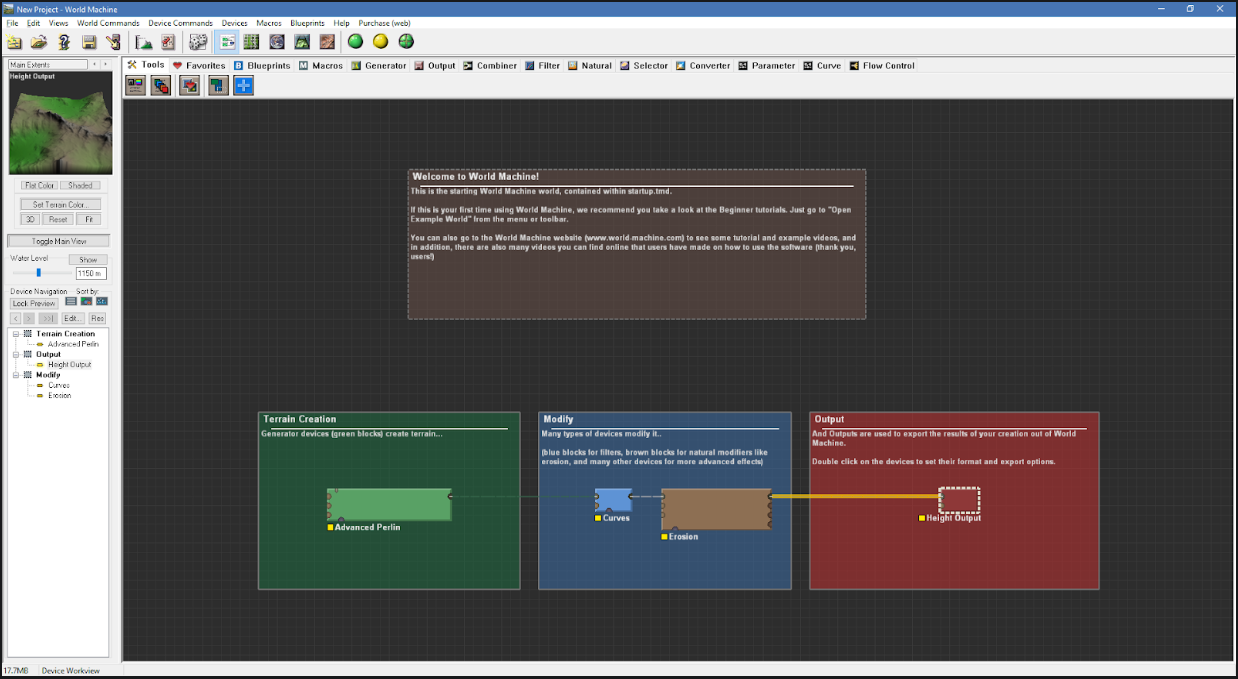
\includegraphics[width=\textwidth,height=\textheight,keepaspectratio]{environments/1.3.png}
\caption{Main screen of World Machine}
\end{figure}
Starting up World machine you are introduced to main screen. You will need to get used to navigating tools around the entire screen. Let’s go through what each section does. 

\subsubsection{Buttons on the Top Bar}
\begin{figure}[H]
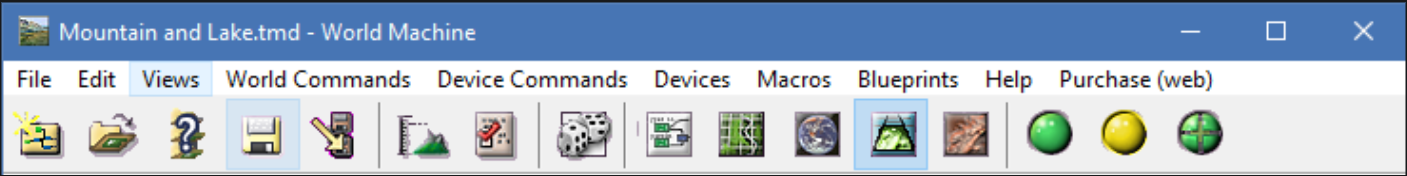
\includegraphics[width=\textwidth,height=\textheight,keepaspectratio]{environments/1.3.1.png}
\caption{Top bar of the main view}
\end{figure}
Located at the top of the window, you’ll find where you can create, load save or export a world, change options for world and exporting, change view port, and finally build, compile the view.
\begin{figure}[H]
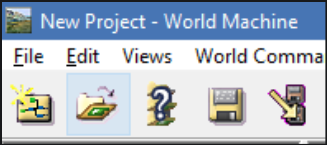
\includegraphics[width=\textwidth,height=\textheight,keepaspectratio]{environments/1.3.2.png}
\caption{New, Open, Example, Save and Export buttons.}
\end{figure}
\begin{itemize}
    \item New
        \begin{itemize}
            \item Creates a new project
        \end{itemize}
    \item Open
        \begin{itemize}
            \item Open a saved project
        \end{itemize}
    \item Example
        \begin{itemize}
            \item Open an examples that demonstrate the capabilities of World Machine
        \end{itemize}
    \item Save
        \begin{itemize}
            \item Save the existing project
        \end{itemize}
    \item Export
        \begin{itemize}
            \item Export files made in the project.
        \end{itemize}
\end{itemize}

\begin{figure}[H]
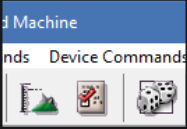
\includegraphics[width=\textwidth,height=\textheight,keepaspectratio]{environments/1.3.3.png}
\caption{Project Settings, World Machine Preferences and Randomizer}
\end{figure}
\begin{itemize}
    \item Project Settings
    \begin{itemize}
        \item Allows you to change settings like Resolution, Map size ( Length and Width) and more.
    \end{itemize}
    \item World Machine Preferences
    \begin{itemize}
        \item Allows you to change how World Machine runs, for example: How many threads and memory is allocated to World Machine, UI settings, Graphics settings and more. (We won’t be touching this, but feel free to change as you see fit)
    \end{itemize}
    \item {Randomiser}
    \begin{itemize}
        \item Selects a random area and setting based on your current project’s build (Tools used in main screen.
    \end{itemize}
\end{itemize}

\subsection{View Modes}
\begin{figure}[H]
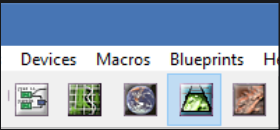
\includegraphics[width=\textwidth,height=\textheight,keepaspectratio]{environments/1.3.4.png}
\caption{Device View, Layout View, Explorer View, 3D View and 2D View}
\end{figure}
\begin{itemize}
    \item Device View
    \begin{itemize}
        \item This changes to the view where you can add devices to shape the terrain
    \end{itemize}
    \begin{figure}[H]
    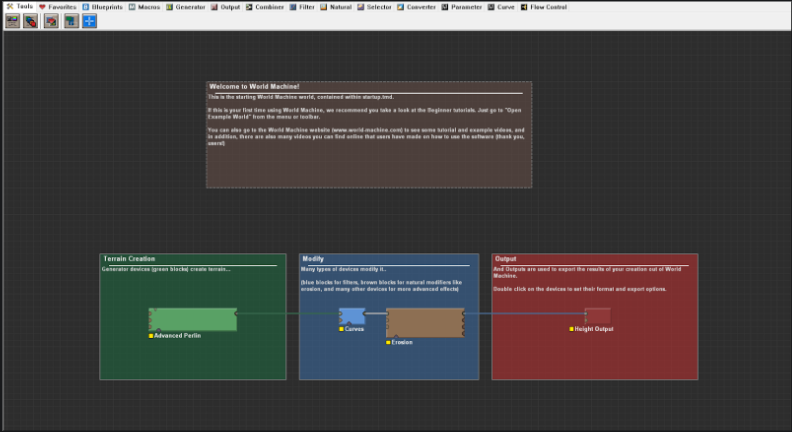
\includegraphics[width=\textwidth,height=\textheight,keepaspectratio]{environments/1.3.5.png}
    \caption{Device View on start up example}
    \end{figure}
    \item Layout View
    \begin{itemize}
        \item Shows a top down view of the environment that is generated in the Device View. This allows you select and view any section of the generated map.
    \end{itemize}
    \begin{figure}[H]
    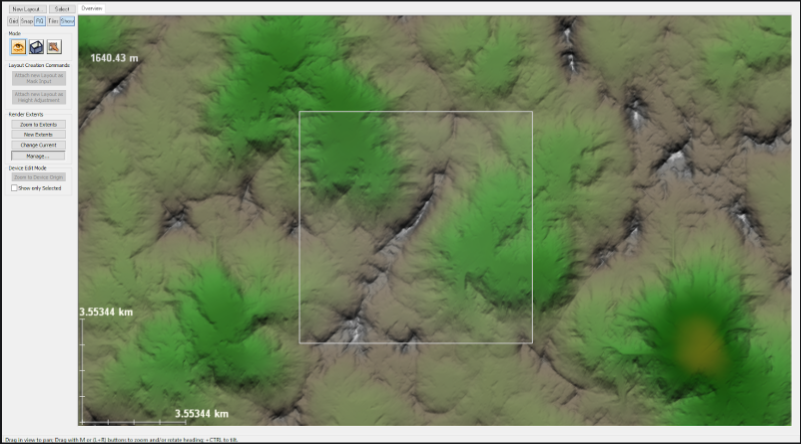
\includegraphics[width=\textwidth,height=\textheight,keepaspectratio]{environments/1.3.6.png}
    \caption{Layout View on start up example}
    \end{figure}
    \item Explorer View
    \begin{itemize}
        \item Shows an angled view of the environment generated from the devices.This view gives you a better view of the generated terrain.
    \end{itemize}
    \begin{figure}[H]
    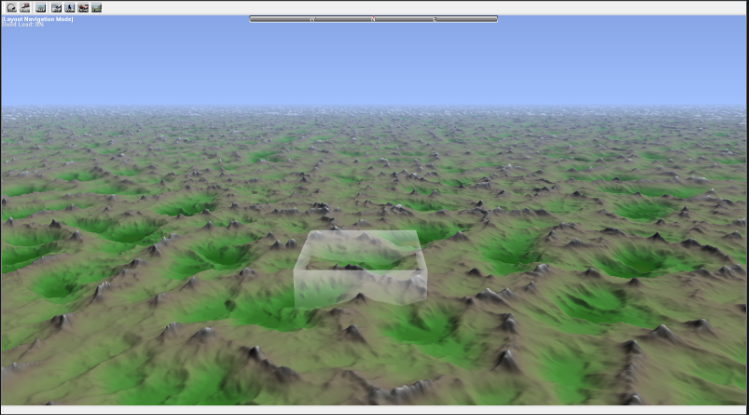
\includegraphics[width=\textwidth,height=\textheight,keepaspectratio]{environments/1.3.7.png}
    \caption{Explorer View on start up example}
    \end{figure}
    \item 3D View
    \begin{itemize}
        \item Shows you the 3d view of the selected terrain you have selected
    \end{itemize}
    \begin{figure}[H]
    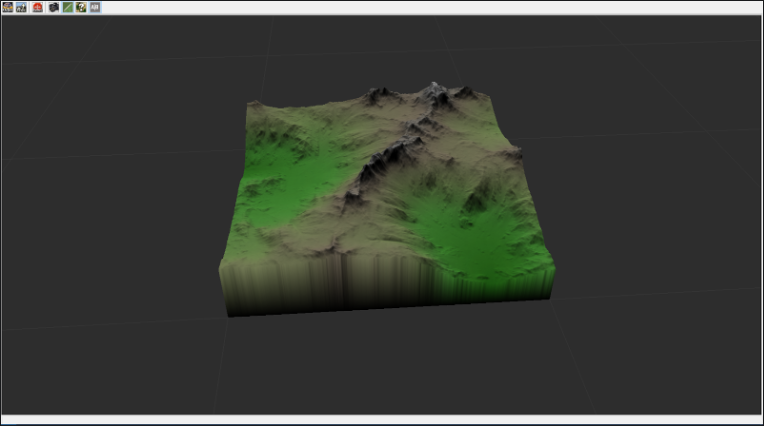
\includegraphics[width=\textwidth,height=\textheight,keepaspectratio]{environments/1.3.8.png}
    \caption{3D View on start up example}
    \end{figure}
    \item 2D View
    \begin{itemize}
        \item Shows you the 2d view of the selected terrain you have selected from above
    \end{itemize}
\end{itemize}
\begin{figure}[H]
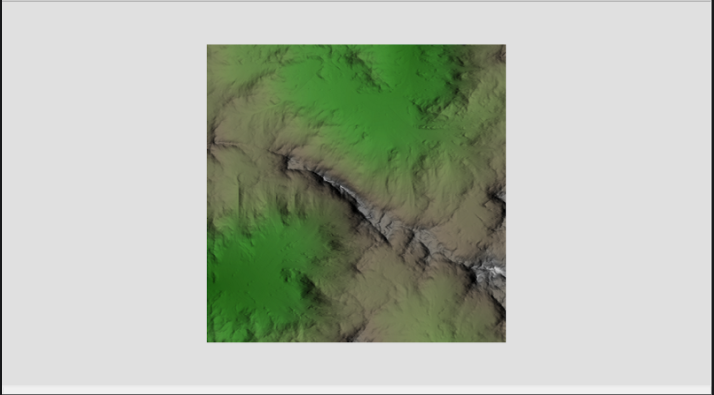
\includegraphics[width=\textwidth,height=\textheight,keepaspectratio]{environments/1.3.9.png}
\caption{2D View on start up example}
\end{figure}
\textit{It is important to note that each view will change based on which device you have selected in the device view or in the sidebar.}

\section{Sculpting a Landscape}
\subsection{Devices and tools}
In this section we’ll be showing you how to create a basic world. Please note this guide does not show you how to use the World machine’s tools to make the exactly what you are looking for, advanced techniques can be found with a quick google search; however, this guide will show you the procedures of building a terrain.
\subsubsection{Generators}
The first step in creating a terrain is selecting a generator; generators are create the initial terrain. Each generator has a different characteristic that gives terrain a unique appearance. To insert a generator go to the Device view in the top bar and then click on Generators in the toolbar
\begin{figure}[H]
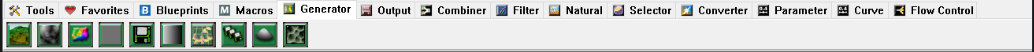
\includegraphics[width=\textwidth,height=\textheight,keepaspectratio]{environments/2.1.1.png}
\caption{Selecting Generators}
\end{figure}
It is here where you can add a generator.
Here is a brief overview of what is possible with each generator:
\begin{itemize}
    \item Advanced Perlin
    \begin{itemize}
        \item Useful for creating large mountains, hills or anything in between. This can be edited by double clicking on the generator to open the settings of that device.
        \item Examples:
    \end{itemize}
\end{itemize}
\begin{figure}[H]
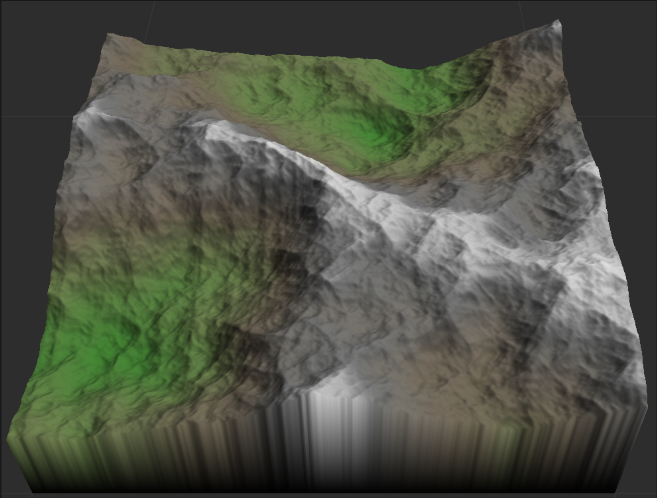
\includegraphics[width=\textwidth,height=\textheight,keepaspectratio]{environments/2.1.2.png}
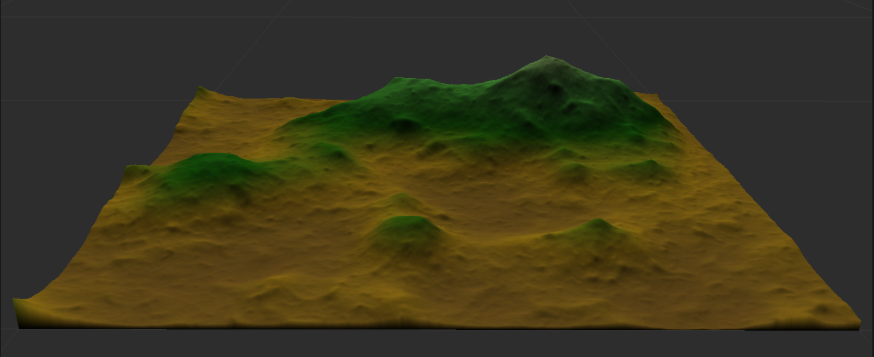
\includegraphics[width=\textwidth,height=\textheight,keepaspectratio]{environments/2.1.3.png}
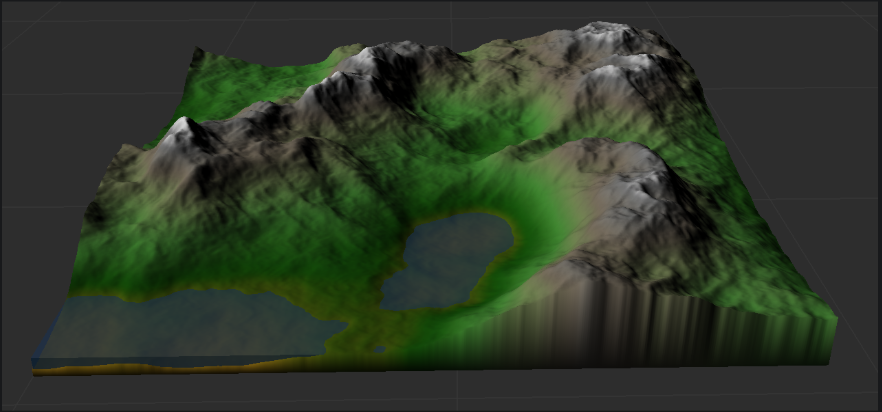
\includegraphics[width=\textwidth,height=\textheight,keepaspectratio]{environments/2.1.4.png}
\caption{Examples of Advanced Perlin - Rocky hills (Top) - Large mountains (Bottom)}
\end{figure}
\begin{figure}[H]
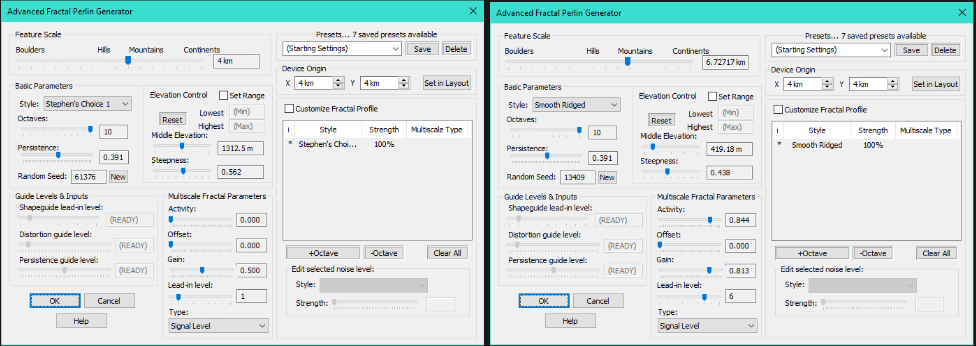
\includegraphics[width=\textwidth,height=\textheight,keepaspectratio]{environments/2.1.5.png}
\caption{Settings for Examples of Advanced Perlin - Rocky hills (Left) - Large mountains (Right)}
\end{figure}
\begin{itemize}
    \item Voronoi Generator
    \begin{itemize}
        \item Useful to create hills and dunes
        \item Examples:
    \end{itemize}
\end{itemize}
\begin{figure}[H]
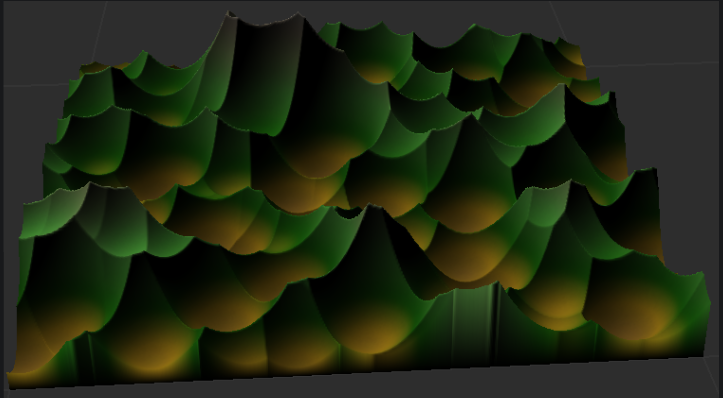
\includegraphics[width=\textwidth,height=\textheight,keepaspectratio]{environments/2.1.6.png}
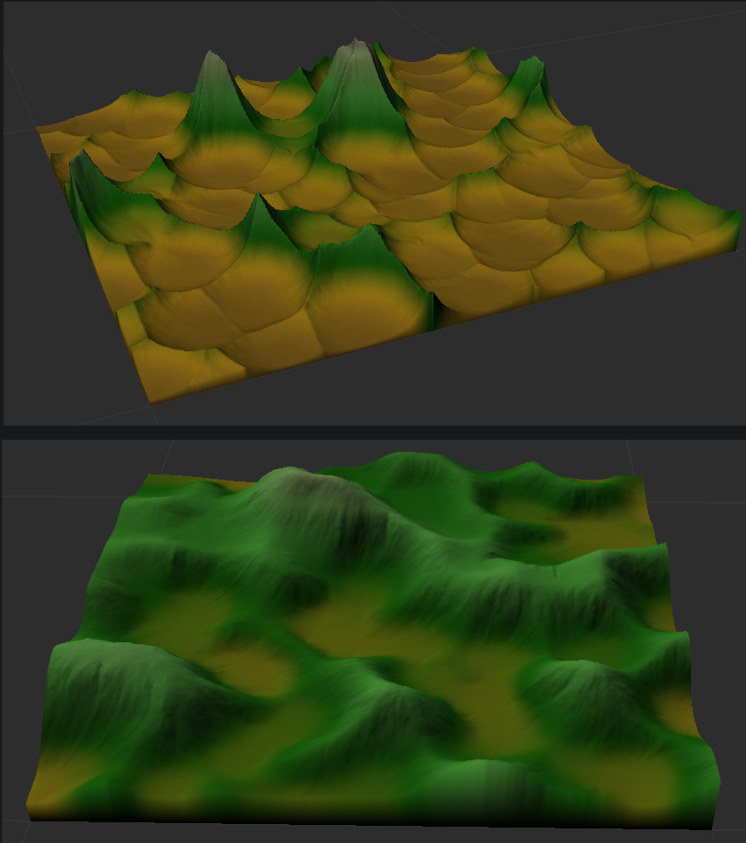
\includegraphics[width=\textwidth,height=\textheight,keepaspectratio]{environments/2.1.7.png}
\end{figure}
\subsection{Creating a desert}
There are many ways to create an environment in World Machine, however in this guide, I will show the methodology used to create the desert environment in this project.
Here is the overall structure for this environment.
\begin{figure}[H]
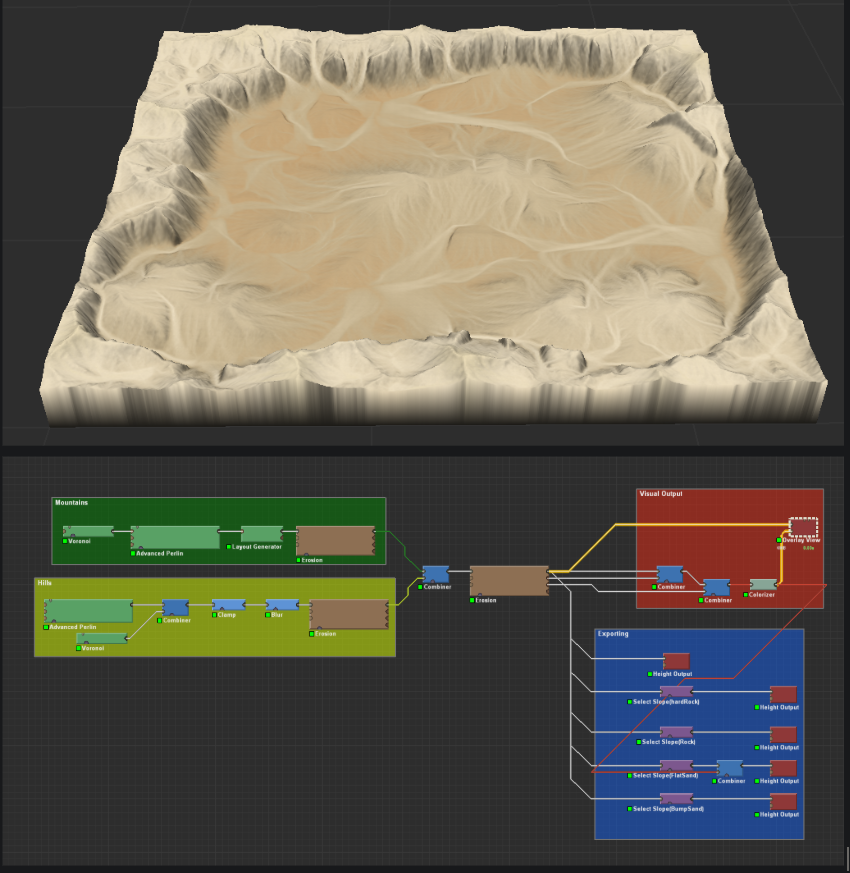
\includegraphics[width=\textwidth,height=\textheight,keepaspectratio]{environments/2.1.8.png}
\end{figure}
\subsubsection{Creating the foundation of the terrain}
Here we split the overall environment into 2 sections. Mountains/Hills and the general landscape. Mountains and Hills allow us to add specific areas that need to be elevated.
Overall Landscape allows us to give the area a slope or where the high and low points are.
\begin{figure}[H]
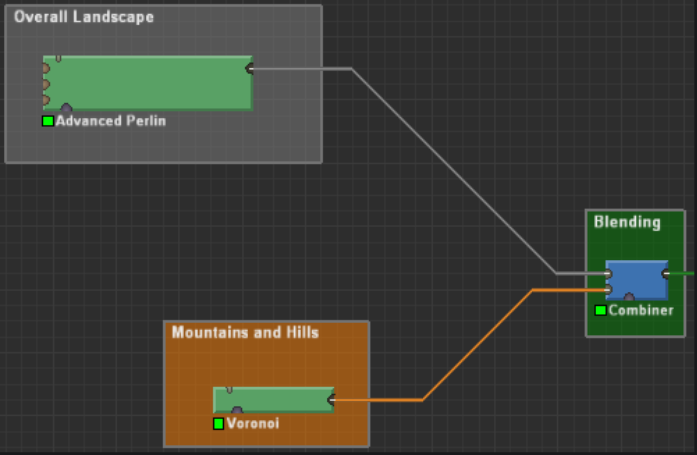
\includegraphics[width=\textwidth,height=\textheight,keepaspectratio]{environments/2.1.9.png}
\end{figure}
\subsection{Overall Landscape}
For this section, it is good to have an idea of the terrain you are trying to create.
Ask yourself, are you building an area that is relatively flat? Do you want to build an area that is in a valley? Or perhaps it is a beach or lake?
Once you have an idea of what you want, you can start trying different generators until you get your desired terrain. Here are some examples:

\subsubsection{Constant:}
\begin{figure}[H]
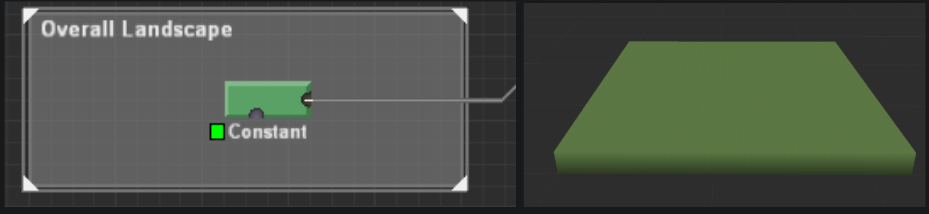
\includegraphics[width=\textwidth,height=\textheight,keepaspectratio]{environments/2.1.10.png}
\end{figure}
Using a constant allows us to create a flat area. The elevation of this land can be adjusted by changing its properties (double click).
\begin{figure}[H]
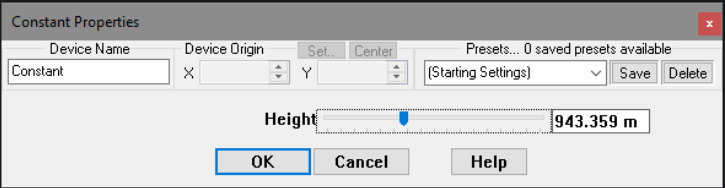
\includegraphics[width=\textwidth,height=\textheight,keepaspectratio]{environments/2.1.11.png}
\end{figure}

\subsubsection{Gradient (Valley and Hills):}
\begin{figure}[H]
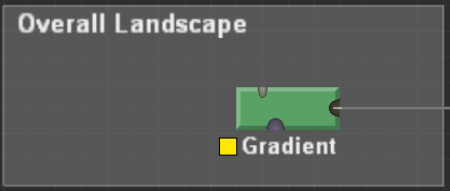
\includegraphics[width=\textwidth,height=\textheight,keepaspectratio]{environments/2.1.12.png}
\end{figure}
Using the gradient tool to build slopes, valleys.
\begin{figure}[H]
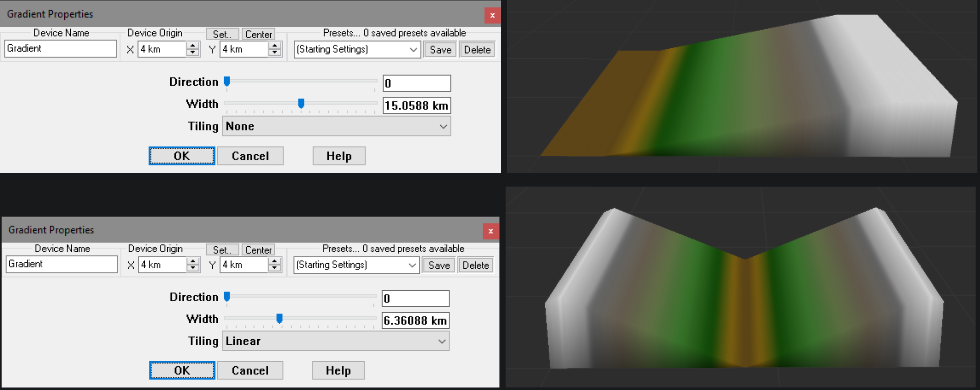
\includegraphics[width=\textwidth,height=\textheight,keepaspectratio]{environments/2.1.13.png}
\end{figure}
\subsubsection{Combination:}
\begin{figure}[H]
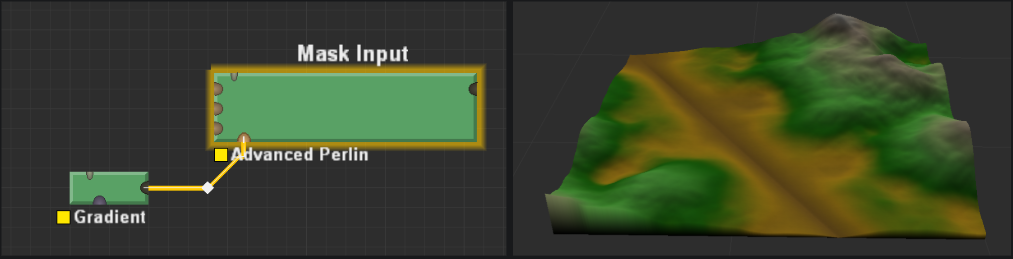
\includegraphics[width=\textwidth,height=\textheight,keepaspectratio]{environments/2.1.14.png}
\end{figure}
It is also possible to add more detail to your overall landscape by connecting a generator another component using the Mask Input, located at the bottom of a component.

\subsection{Mountains and Hills}
This adds detail to the map as well as emphasize a particular bio-me.
\subsubsection{Advanced Perlin:}
This is very useful to create large rounder mountains.
\begin{figure}[H]
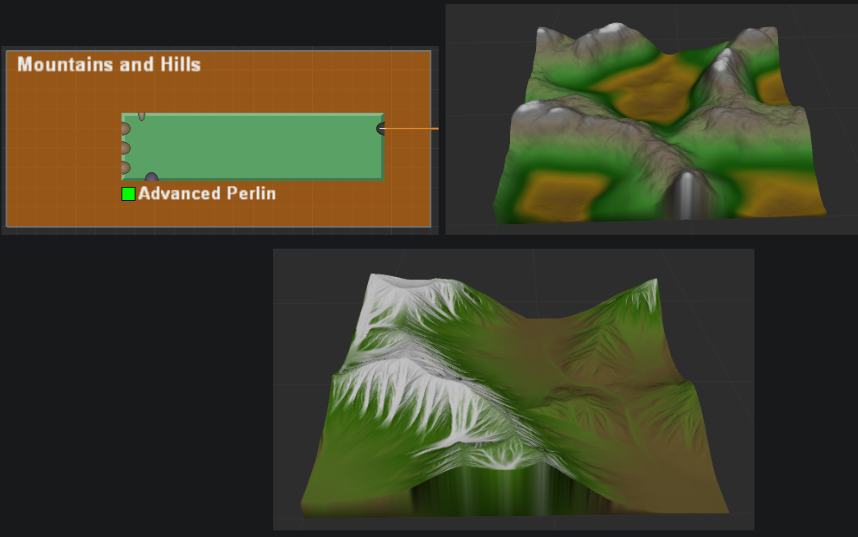
\includegraphics[width=\textwidth,height=\textheight,keepaspectratio]{environments/2.1.15.png}
\end{figure}
\subsubsection{Voronoi:}
Voronoi allows you to create sharp and complex mountains. A very quick way to create multiple mountains that are connected together.
\begin{figure}[H]
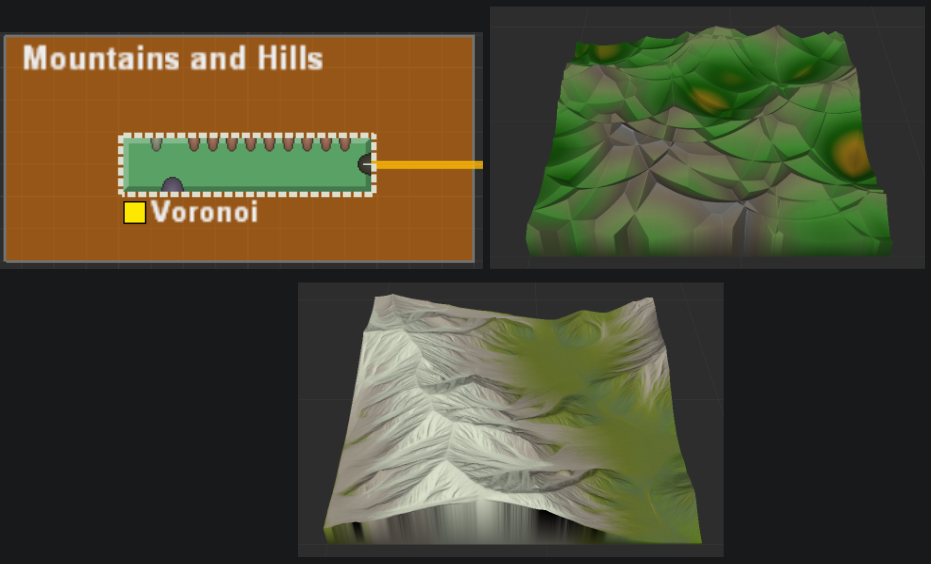
\includegraphics[width=\textwidth,height=\textheight,keepaspectratio]{environments/2.1.16.png}
\end{figure}

\subsubsection{Basic Noise:}
Basic noise is quite flexible to create mountains similar to Advanced Perlin, but it also allows you to create more abstract rock formations, like craters and plateaus.
\begin{figure}[H]
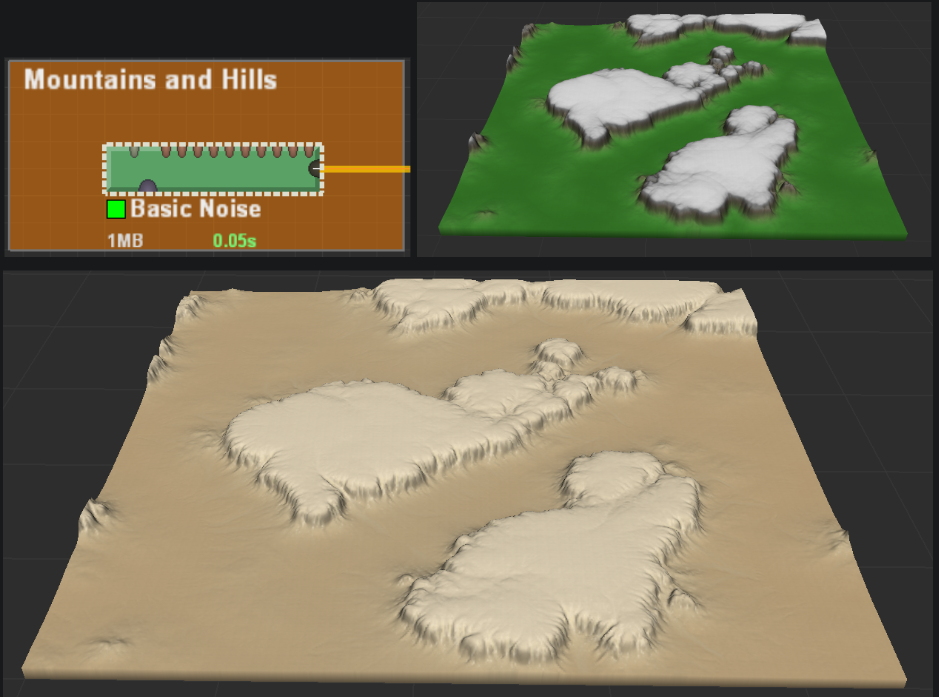
\includegraphics[width=\textwidth,height=\textheight,keepaspectratio]{environments/2.1.17.png}
\end{figure}

\subsection{Blending:}
Using the combiner tool is optional, however this allows us to blend the two landscapes together to give the overall structure of one whilst retaining the interesting sections of the other.
There are different ways to combine the 2 together, play around with each method and settings until you find something you’re happy with.
\begin{figure}[H]
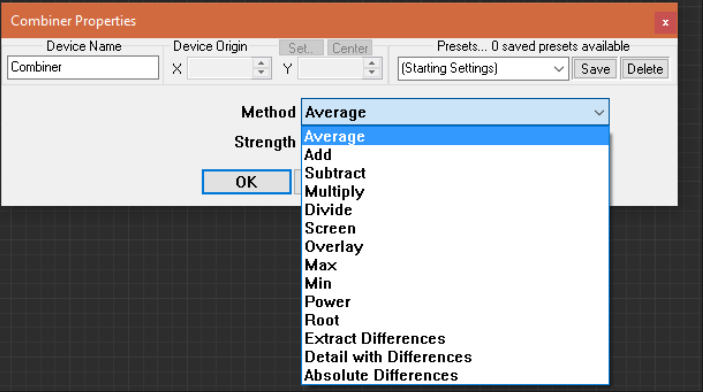
\includegraphics[width=\textwidth,height=\textheight,keepaspectratio]{environments/2.1.18.png}
\end{figure}

\subsection{Example}:
For project’s desert map, it was my decision to create an area that has both a large open space but also have a hill and a tight corner that could something could be hidden behind.
Starting with the overall landscape, I was seeking for a desert environment has a mixture of low and gentle hills; which is why I used an advanced perlin with the following settings.
\begin{figure}[H]
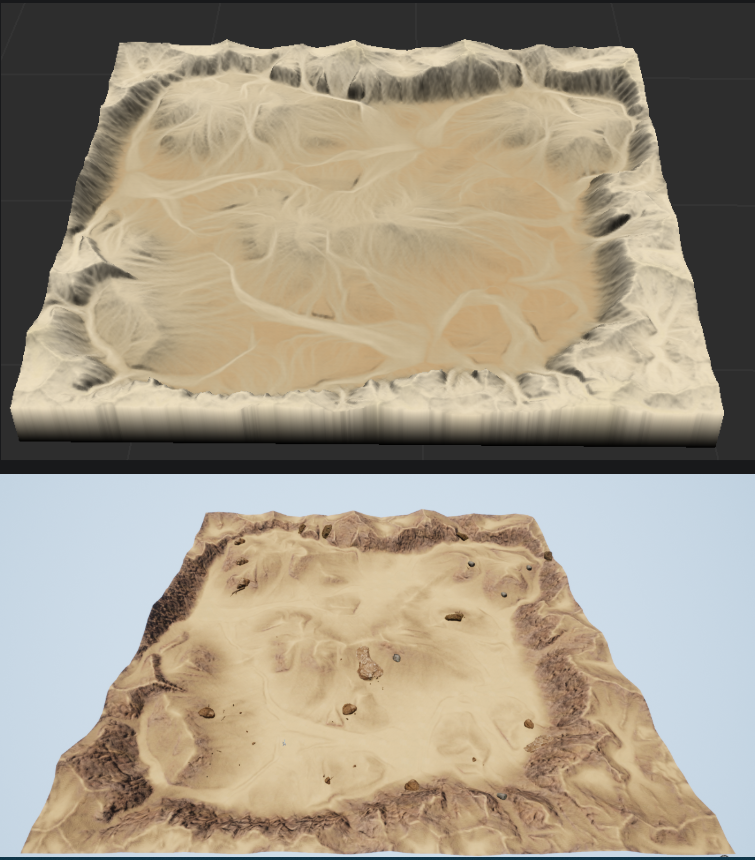
\includegraphics[width=\textwidth,height=\textheight,keepaspectratio]{environments/2.1.19.png}
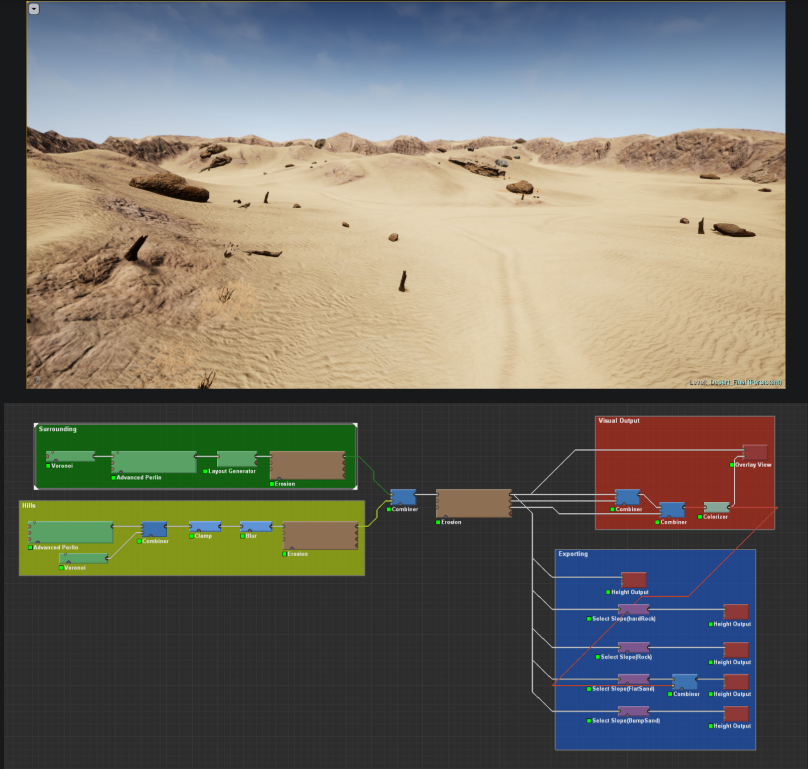
\includegraphics[width=\textwidth,height=\textheight,keepaspectratio]{environments/2.1.20.png}
\end{figure}
\section{Export from World Machine}
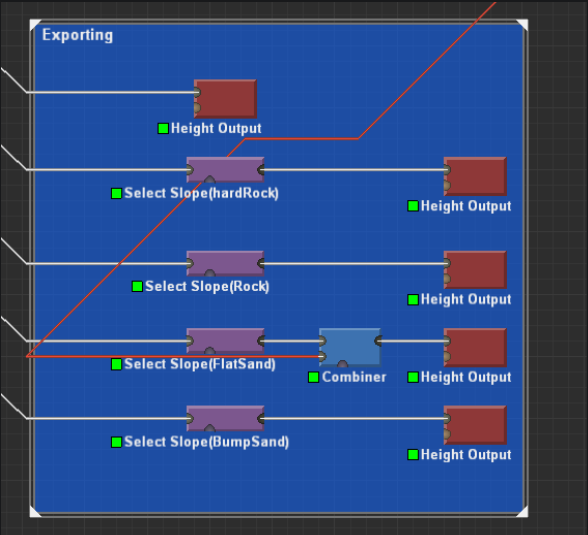
\includegraphics[width=\textwidth,height=\textheight,keepaspectratio]{environments/3.1.png}
Here is an overview of the devices needed to import the map we created to Unreal Engine

\subsection{Creating Height maps}
To export the overall geometry of the environment we will need a “Height Output” device, located in output tab. Connect the Height Output to the output of the last device of the terrain you have created (This excludes the Visual devices).
 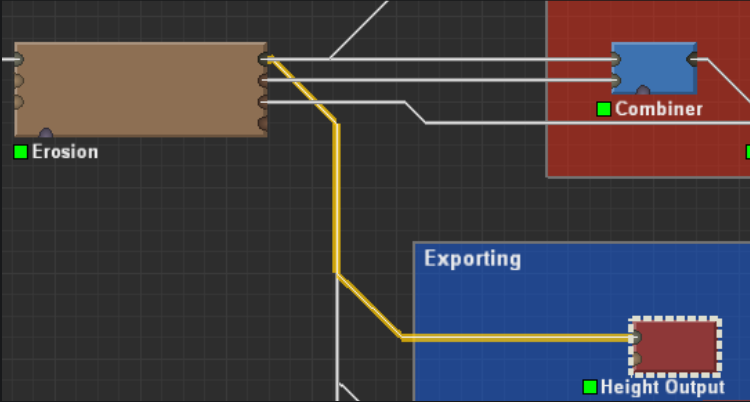
\includegraphics[width=\textwidth,height=\textheight,keepaspectratio]{environments/3.1.1.png}
Now we need to export the height map to the right file type. Double click on Height Output and give a name to the file and set the File format to RAW16. You’ll also need to set the file path of where the file will be exported to, this is done by clicking on the “Set” button.
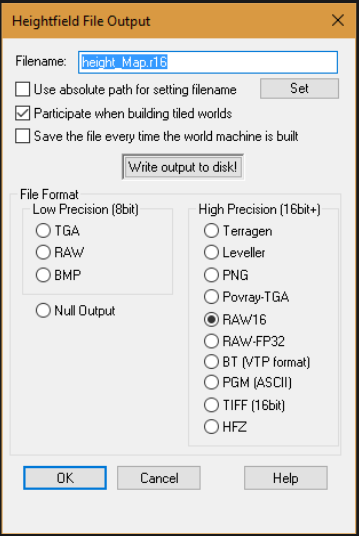
\includegraphics[width=\textwidth,height=\textheight,keepaspectratio]{environments/3.1.2.png}
Once that is set up, build the world then you can click on the “Write output to disk” button and it will create a file.

\subsection{Creating Alpha Maps}
Alpha Maps are used to tell the Unreal Engine where to paint specific textures on the landscape that you have created. This significantly enhances the visual appearance of the landscape when importing into Unreal Engine. We will need to export individual images of each material we want to use. Sadly we can’t just import World Machine colorizer directly since World Machine’s colouring is incompatible with Unreal Engine’s system.

Here we can use a range of devices from the Selector Tab to choose a specific angle of a slope or the height of the terrain. Attach the input of each device to the primary output of the terrain and the output of the selector device to another individual Height Output.
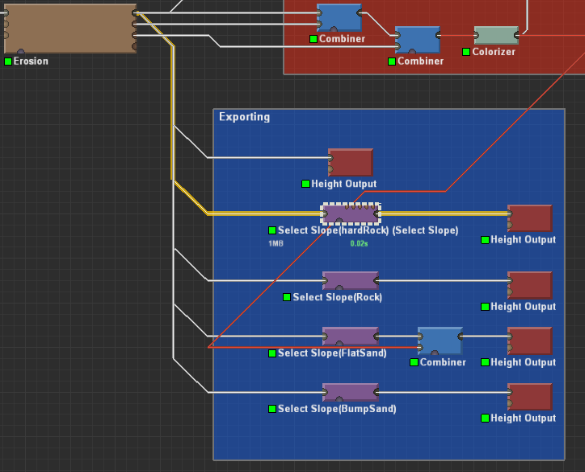
\includegraphics[width=\textwidth,height=\textheight,keepaspectratio]{environments/3.2.1.png}
In general, you will want to plan out what type of texture you want on your map (In the case of the example, there are 4 types of materials) then work out where you want each texture be painted. You want to make sure you cover every space on the map. White represents where the material will be painted.
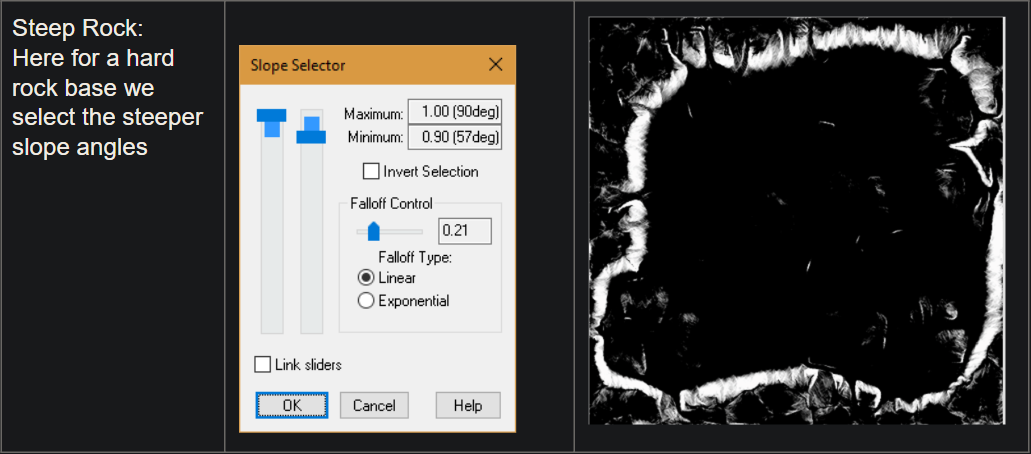
\includegraphics[width=\textwidth,height=\textheight,keepaspectratio]{environments/3.2.2.png}
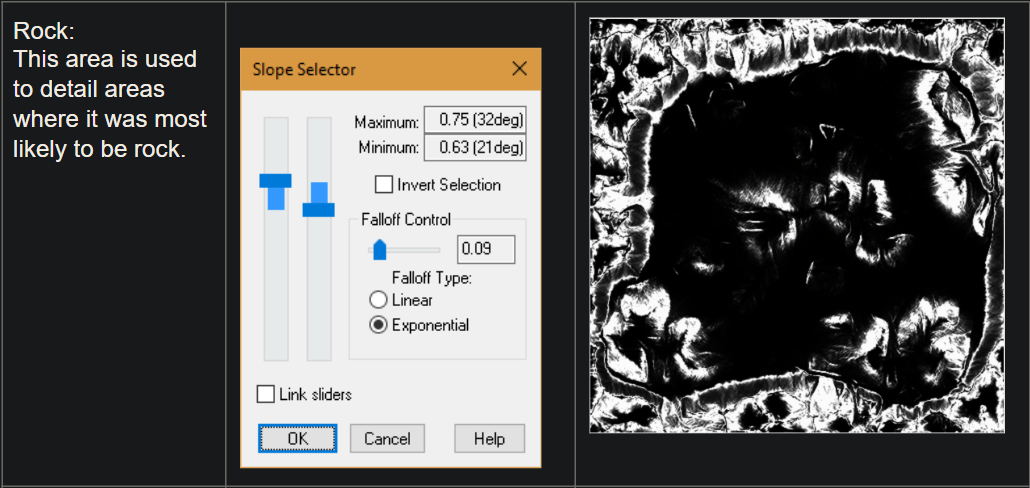
\includegraphics[width=\textwidth,height=\textheight,keepaspectratio]{environments/3.2.3.png}
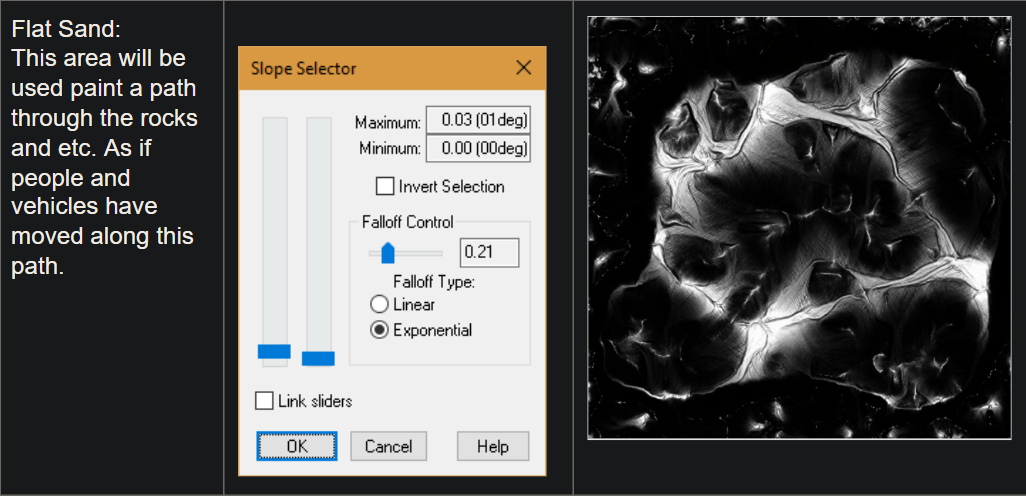
\includegraphics[width=\textwidth,height=\textheight,keepaspectratio]{environments/3.2.4.png}
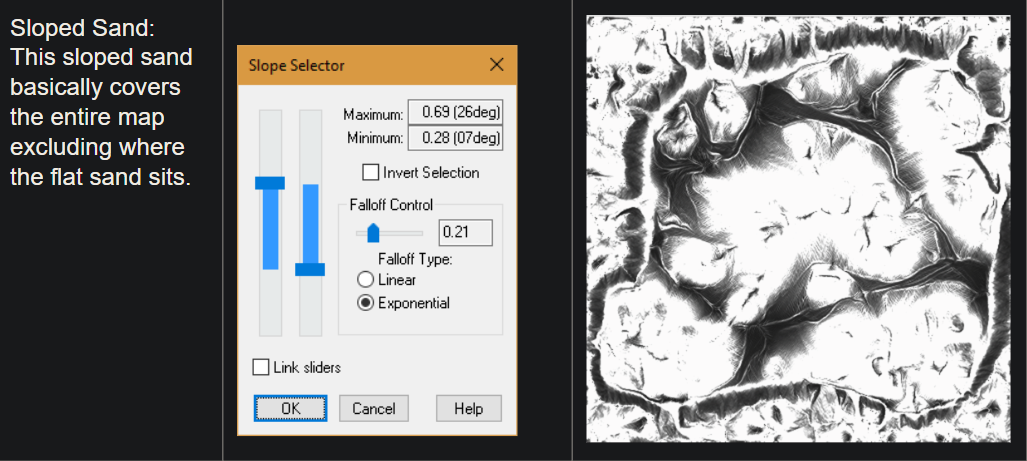
\includegraphics[width=\textwidth,height=\textheight,keepaspectratio]{environments/3.2.5.png}
For each selector tool you will want to configure the Height Output device settings, just like in the previous chapter.
Create a file name, then set the export directory, the select PNG as the file format.
Once you’re happy with your selector settings, build the world then you can write output to disk.
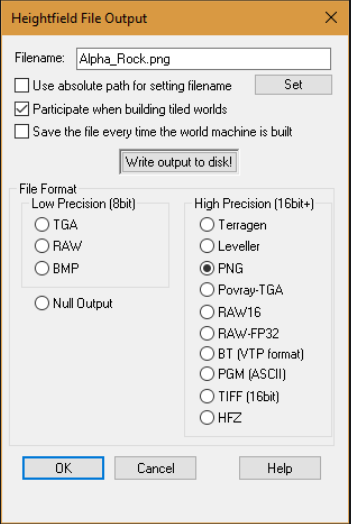
\includegraphics[width=\textwidth,height=\textheight,keepaspectratio]{environments/3.2.6.png}
Very quickly you can simply click on Export Terrain icon  in the top bar to quickly export all outputs to disk.
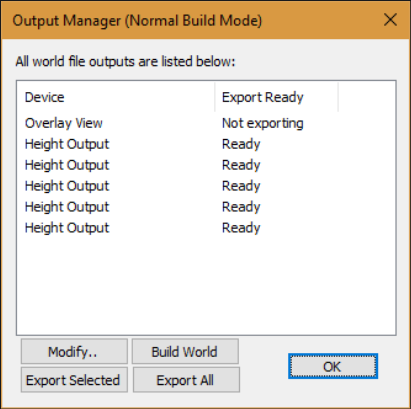
\includegraphics[width=\textwidth,height=\textheight,keepaspectratio]{environments/3.2.7.png}

\section {Creating a Material in Unreal Engine}
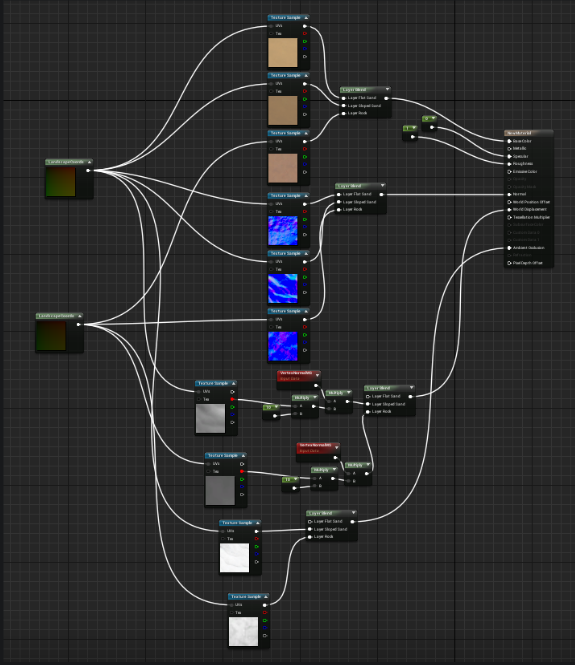
\includegraphics[width=\textwidth,height=\textheight,keepaspectratio]{environments/4.1.png}
To create a new material, go to the content browser and right click and click on material under Create Basic Asset, then double click on the new material.
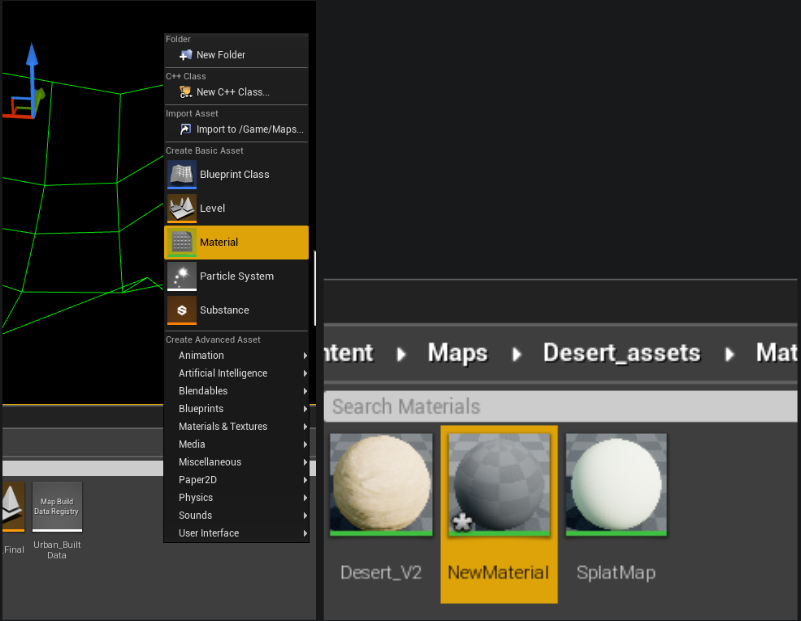
\includegraphics[width=\textwidth,height=\textheight,keepaspectratio]{environments/4.2.png}
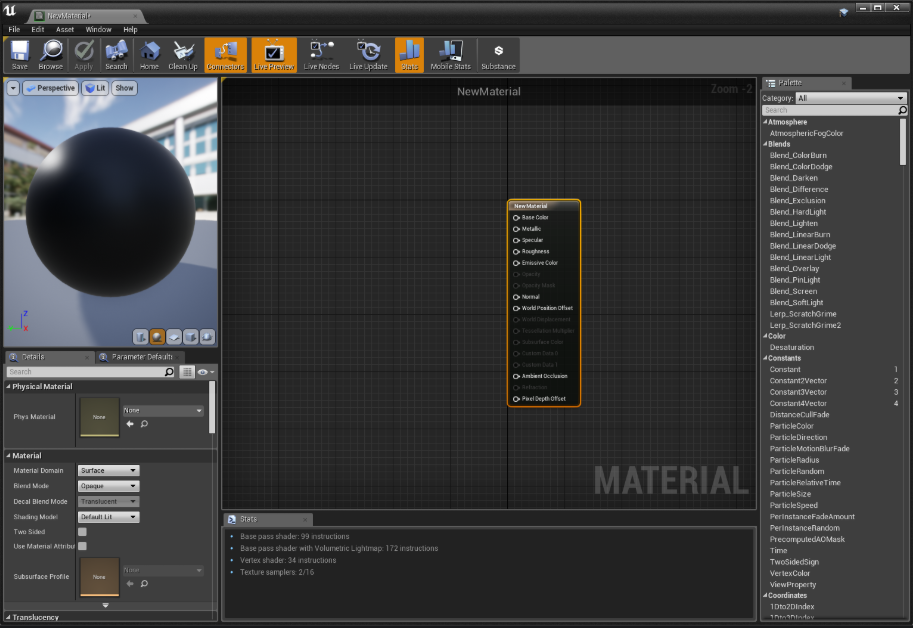
\includegraphics[width=\textwidth,height=\textheight,keepaspectratio]{environments/4.3.png}
Now in the material editor, you’ll need to decide all the layers of materials you’ll want in your level. For example, a forest environment may want to have grass, dirt, gravel and sand; for the desert map, we want a rock layer, a sloped sand (bumpy looking sand) and flat sand (flattened sand).
To find materials, you can go to websites such as the unreal engine marketplace, or Textures.com, then download all of the images available in the texture page.

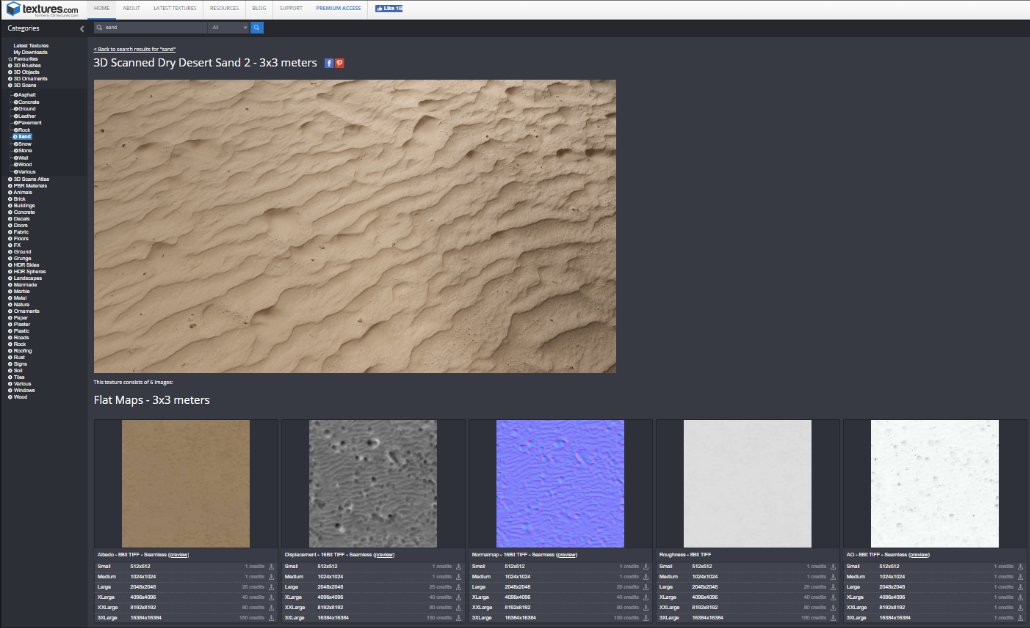
\includegraphics[width=\textwidth,height=\textheight,keepaspectratio]{environments/4.4.png}
Once you have decided what layers you want, right click on an empty space in the material editor, and type LayerBlend and click on the LandscapeLayerBlend under Landscape.

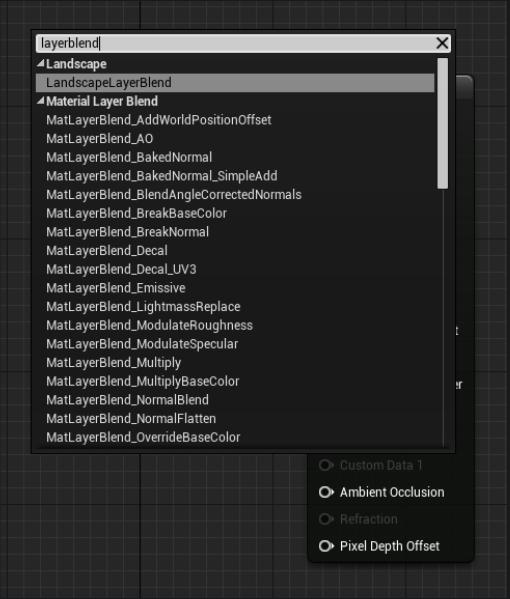
\includegraphics[width=\textwidth,height=\textheight,keepaspectratio]{environments/4.5.png}
Once added, click on the module and on the left hand side click on the “+” next to 0 Array Elements. This will add a layer to the material; click the + sign as many times as many layers you want, for our case we’ll have 3 layers.
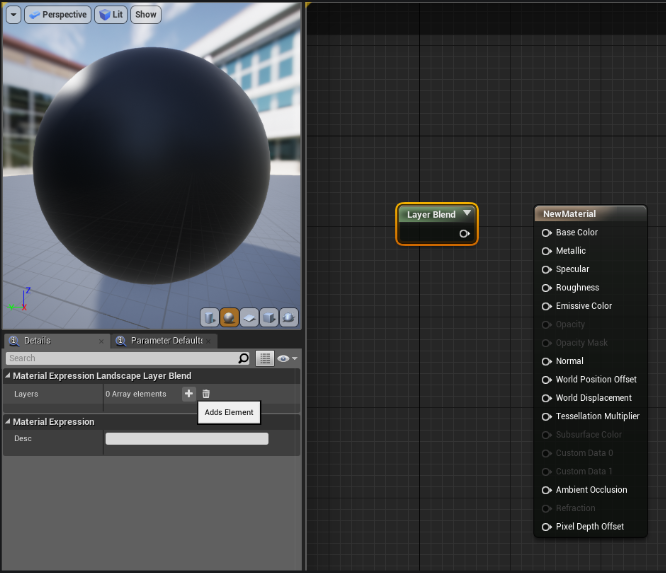
\includegraphics[width=\textwidth,height=\textheight,keepaspectratio]{environments/4.6.png}
Expand each layer and give each layer a name and make sure each Blend Type is “LB Weight Blend”.
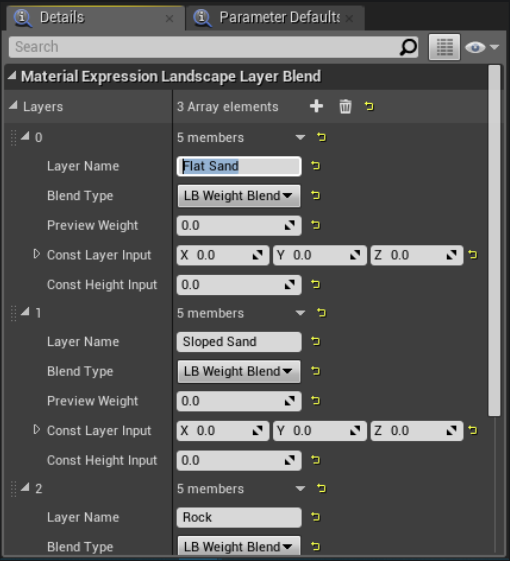
\includegraphics[width=\textwidth,height=\textheight,keepaspectratio]{environments/4.7.png}
The thing you need to consider is the preview weight, this determines which material take presence when painting. For example, we have a rock and sand layer where the rock should be underneath the sand; therefore if the sand and rock textures overlap at a point, the sand will be more prevalent than the rock.
It is a bit of playing around but if unsure just set everything to 0.5 then adjust it later.
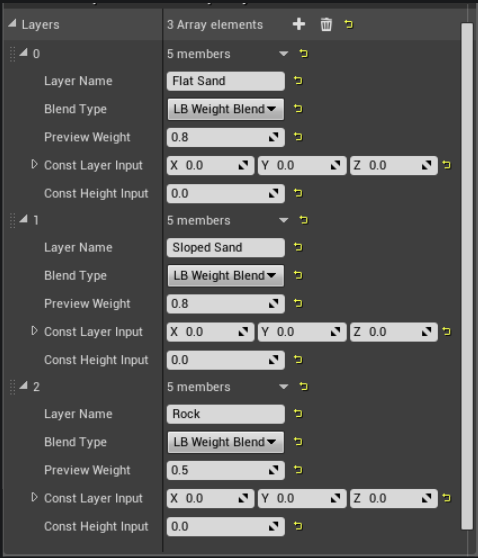
\includegraphics[width=\textwidth,height=\textheight,keepaspectratio]{environments/4.7-2.png}
Once you have this it’s time to connect up the materials.
Click and drag Albedo images from the content browser into the material editor.
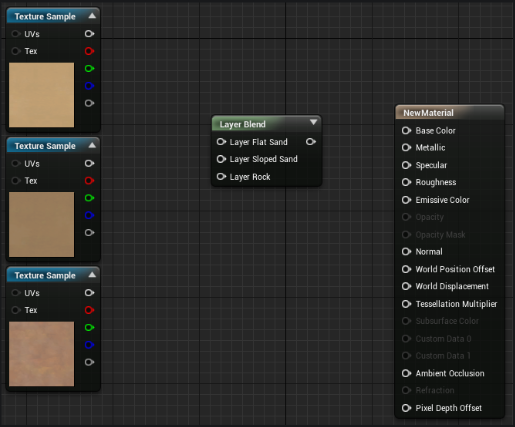
\includegraphics[width=\textwidth,height=\textheight,keepaspectratio]{environments/4.8.png}
You can also just add a colour as a Albedo image by right clicking a blank area and typing constant then select the “Constant3Vector”.
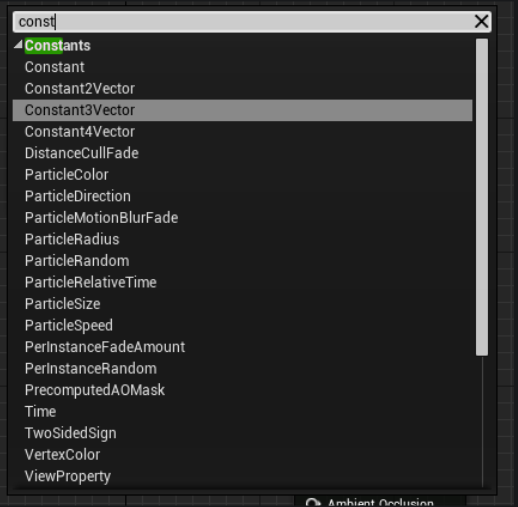
\includegraphics[width=\textwidth,height=\textheight,keepaspectratio]{environments/4.9.png}
Double click on the Constant3Vector device and select a colour that you want.
\includegraphics[width=\textwidth,height=\textheight,keepaspectratio]{environments/4.10.png}
Continuing on you can now connect each device together as shown.
\includegraphics[width=\textwidth,height=\textheight,keepaspectratio]{environments/4.11.png}
This now shows colour on your texture. You can now follow a similar procedure for normal and ambient occlusion images.
\includegraphics[width=\textwidth,height=\textheight,keepaspectratio]{environments/4.12.png}
For Specular and Roughness, you can follow the same procedure as above if there are images that you can use; otherwise you can set each value with a constant device to reduce the shininess of the material.
For height/displacement images, you will need to click on the main material device and navigate to the details window and find the Tessellation section. Select “Flat Tessellation” for the mode.
 \includegraphics[width=\textwidth,height=\textheight,keepaspectratio]{environments/4.13.png}
Once selected, you can copy the following:
\includegraphics[width=\textwidth,height=\textheight,keepaspectratio]{environments/4.14.png}
I’ll be quite honest, I’m not sure what or why it works but I found a YouTube video called “Landscape Material Tutorial - Adding Tessellation (Unreal Engine 4)” was quite useful for a more in depth guide to adding tessellation.
\textbf{https://www.youtube.com/watch?v=W1MRDXUWID4}
That is basically how you create a basic material in unreal engine. Of course there are more advanced ways to get exactly what you want, but this should suffice for beginning.
\subsection{Scaling Textures/Materials}
So you may have noticed that your material is very small or it’s repeating when you use it in your map, and it doesn’t look very nice.
\includegraphics[width=\textwidth,height=\textheight,keepaspectratio]{environments/4.15.png}
To fix this we will need to add Landscape Layer Coords devices.
\includegraphics[width=\textwidth,height=\textheight,keepaspectratio]{environments/4.16.png}
From this we can increase the mapping scale to make the textures scale larger across the environment.
\includegraphics[width=\textwidth,height=\textheight,keepaspectratio]{environments/4.17.png}
Finally connect the device to the UVs of the each texture image.
\includegraphics[width=\textwidth,height=\textheight,keepaspectratio]{environments/4.18.png}
You can also add multiple Landscape layer coords for each texture.
\includegraphics[width=\textwidth,height=\textheight,keepaspectratio]{environments/4.19.png}
\includegraphics[width=\textwidth,height=\textheight,keepaspectratio]{environments/4.20.png}

\section {Import to Unreal Engine}
Now is the time to import the height map and alpha maps to the unreal engine to create a usable world.
Open up Unreal engine and create a new level. This can be done by going to the content browser and right click an empty space and click on Level, as shown:
\includegraphics[width=\textwidth,height=\textheight,keepaspectratio]{environments/5.1.png}
Give the file a name and then double click on it.
\includegraphics[width=\textwidth,height=\textheight,keepaspectratio]{environments/5.2.png}
The level will open to a black empty space. Navigate to the Modes window 
\includegraphics[width=\textwidth,height=\textheight,keepaspectratio]{environments/5.3.png}
If your Mode window is missing, go to the very top, click on windows and then click on modes.
\includegraphics[width=\textwidth,height=\textheight,keepaspectratio]{environments/5.4.png}
When shown the Modes window, go to Landscape, or press Shift+3
\includegraphics[width=\textwidth,height=\textheight,keepaspectratio]{environments/5.5.png}
Once open, click on the manage tab then select “Import from File” under New Landscape. Then click on the “...” button beside the Height map File text box.
\includegraphics[width=\textwidth,height=\textheight,keepaspectratio]{environments/5.6.png}
Here you want to navigate to your height map file, which you created in chapter 3.1. 
\includegraphics[width=\textwidth,height=\textheight,keepaspectratio]{environments/5.7.png}
Once opened, you’ll see a very basic mesh of your world; don’t worry it’ll look better later.
\includegraphics[width=\textwidth,height=\textheight,keepaspectratio]{environments/5.8.png}
Next you can adjust the following settings:
\includegraphics[width=\textwidth,height=\textheight,keepaspectratio]{environments/5.9.png}
Now you can finally add your material you made in the previous chapter. Here we will need to create layer info files for each layer.
\includegraphics[width=\textwidth,height=\textheight,keepaspectratio]{environments/5.10.png}
Click on the plus sign and select Weight-Blended Layer( Normal), find a neat place to put them and do this for each layer.
\includegraphics[width=\textwidth,height=\textheight,keepaspectratio]{environments/5.11.png}
After that it’s time to add the Alpha images from chapter 3.2. Click on the “...” button and open the respective alpha image
\includegraphics[width=\textwidth,height=\textheight,keepaspectratio]{environments/5.12.png}
Once each alpha image has been loaded we can finally import the landscape using the “import” button at the bottom.
Now you may notice it’s still black and you can’t see anything.

We need to add lights, go to the modes window and click on the place tab (Shift + 1)

Type in sky and click and drag the “BP_Sky_Sphere” blueprint on to the map. This will give you a sky sphere.
\includegraphics[width=\textwidth,height=\textheight,keepaspectratio]{environments/5.13.png}
You can change the settings of how the sky sphere looks and behaves, like the colour and cloud speeds.
\includegraphics[width=\textwidth,height=\textheight,keepaspectratio]{environments/5.14.png}
So now you can see the terrain but it’s still black.
\includegraphics[width=\textwidth,height=\textheight,keepaspectratio]{environments/5.15.png}
Now head back to the place tab and add a directional light. You can adjust the angle of the shadows by changing the rotation of the directional light.
\includegraphics[width=\textwidth,height=\textheight,keepaspectratio]{environments/5.16.png}
\includegraphics[width=\textwidth,height=\textheight,keepaspectratio]{environments/5.17.png}

Yay, now you can see the map properly, but the map looks way too bumpy. You can go to the world outliner and select the landscape and change the scale numbers, under Transform.
\includegraphics[width=\textwidth,height=\textheight,keepaspectratio]{environments/5.18.png}
\includegraphics[width=\textwidth,height=\textheight,keepaspectratio]{environments/5.19.png}

Now you managed to scale it nicely, you’re probably thinking it’s a still a bit dark with a lot of shadows. Now it’s time to add a sky light to the map.
\includegraphics[width=\textwidth,height=\textheight,keepaspectratio]{environments/5.20.png}
\includegraphics[width=\textwidth,height=\textheight,keepaspectratio]{environments/5.21.png}

Now your map looks a lot better, but we should let the map build and bake the lighting.
Click on the build icon and let the computer do its job for awhile.
\includegraphics[width=\textwidth,height=\textheight,keepaspectratio]{environments/5.22.png}
Go ahead and play around with the Details settings until you’re happy.

\section {Adding Foliage and Objects}
\subsection{Adding Foliage}
To add foliage, head over the to mode window and click on the Foliage tab (Shift + 4)
\includegraphics[width=\textwidth,height=\textheight,keepaspectratio]{environments/6.1.1.png}
Here you will need to add all the assets that you want to decorate the world with.
Go to your content browser then select and drag all the models you want into the mode window.
\includegraphics[width=\textwidth,height=\textheight,keepaspectratio]{environments/6.1.2.png}
Once they’re in the Foliage area, select one, or many of the objects and change the settings to make it look spawn in a random orientation or different sizes and such.
\includegraphics[width=\textwidth,height=\textheight,keepaspectratio]{environments/6.1.3.png}
You can also change whether a object can be collided with. For Grass, you won’t need to do this but for rocks and solid objects you will want to select “BlockAll” for Collision Presets. 
\includegraphics[width=\textwidth,height=\textheight,keepaspectratio]{environments/6.1.4.png}
You can save some performance by adjusting the culling distance of foliage.
\includegraphics[width=\textwidth,height=\textheight,keepaspectratio]{environments/6.1.5.png}
This makes object disappear depending how far away they are from the player.
To paint an object, simply move your mouse in the view port and click and drag where you want to add the foliage.
\includegraphics[width=\textwidth,height=\textheight,keepaspectratio]{environments/6.1.6.png}

You can change how you paint the foliage by adjusting the settings at the top of the modes window.
\includegraphics[width=\textwidth,height=\textheight,keepaspectratio]{environments/6.1.7.png}
If you went a bit too crazy, you can remove objects by holding down Shift and then Left click to remove any foliage that’s in the area of effect.
\includegraphics[width=\textwidth,height=\textheight,keepaspectratio]{environments/6.1.8.png}
When you’re done with add that object, you can deselect the object.
\includegraphics[width=\textwidth,height=\textheight,keepaspectratio]{environments/6.1.9.png}

\subsection{Adding objects}
You will need to add objects that are not apart of foliage. Things like player starting points, buildings, interact-able objects and NPCs need to be added as an object.
To do this you can simply find your object in the content browser or in the Place tab and click and drag into the view port.
\includegraphics[width=\textwidth,height=\textheight,keepaspectratio]{environments/6.2.1.png}

\end{document}